\documentclass{article}
\usepackage[utf8]{inputenc}
\usepackage{verbatim}
\usepackage{kotex}
\usepackage{graphicx}
\usepackage{subfigure}
\usepackage{caption}
\title{PL HW2 Project}
\author{승완 김}
\date{April 2023}

\begin{document}
\title{HW2}
\author{B831051 김승완}
\date{April 2023}
\maketitle


\section{동작 방식에 대한 간단 설명}
lex는 Lexical Analyzer Generator로, 파일들을 읽어들여 문자들을 토큰으로 분리하는 기능을 한다. l 확장자의 파일에 정규 표현식(Regular Expression)으로 된 pattern과 이에 따라 동작하는 코드(이는 c언어의 코드로 구현됨)를 action에 기술해줘야 한다. l 확장자 파일은 정의절, 규칙절, 그리고 사용자 서브루틴절로 이루어진다. 정의절에서는 C언어 코드에서의 출력을 위한 헤더파일을 끌어올 수 있으며 변수의 선언을 할 수 있다. 정의절이 끝난 아래 부분에서는 규칙절, 서브루틴절에서 편리하게 사용할 수 있는 일종의 alias를 선언할 수 있다. 규칙절에는 input으로 들어오는 파일의 문자들이 토큰으로 묶여진다. pattern을 정규 표현식을 사용해서 기술하고 난 이후에는 action을 통해 원하는 c코드 명령어를  기술한다. 마지막으로 사용자 서브루틴 절에서는 lex.yy.c 파일의 마지막 부분에 그대로 복사된다. 서브루틴 절의 int main()부분에서는 yylex()함수를 가동시켜줌으로써 스트림을 통해 읽어들일 수 있도록 한다. 또한 파일의 끝, 즉 EOF를 만나면 yywrap()함수를 자동으로 호출하는데 이를 위해 int main()부의 다음에 int wrap() 역시 정의해주어야 한다. 
\newline
이렇게 작성된 확장자의 파일은 lex 명령어를 통해서 lex.yy.c 라는 c확장자의 파일로 한번 컴파일 된다. 이는 다시 cc 명령어(추후에 yacc를 통해서 구현함) 를 통해 cc lex.yy.c -o lex의 방식으로 lex 실행파일이 생성된다. 마지막 명령어는 현재 위치의 lex 실행파일에 input 파일을 적용하기 위한 것으로써, ./lex < test.c를 통해 구현된다. 
\newline\newline\newline\newline\newline\newline\newline\newline
\newline\newline
\section{실행 결과 이미지}
\begin{figure}
    \centering
    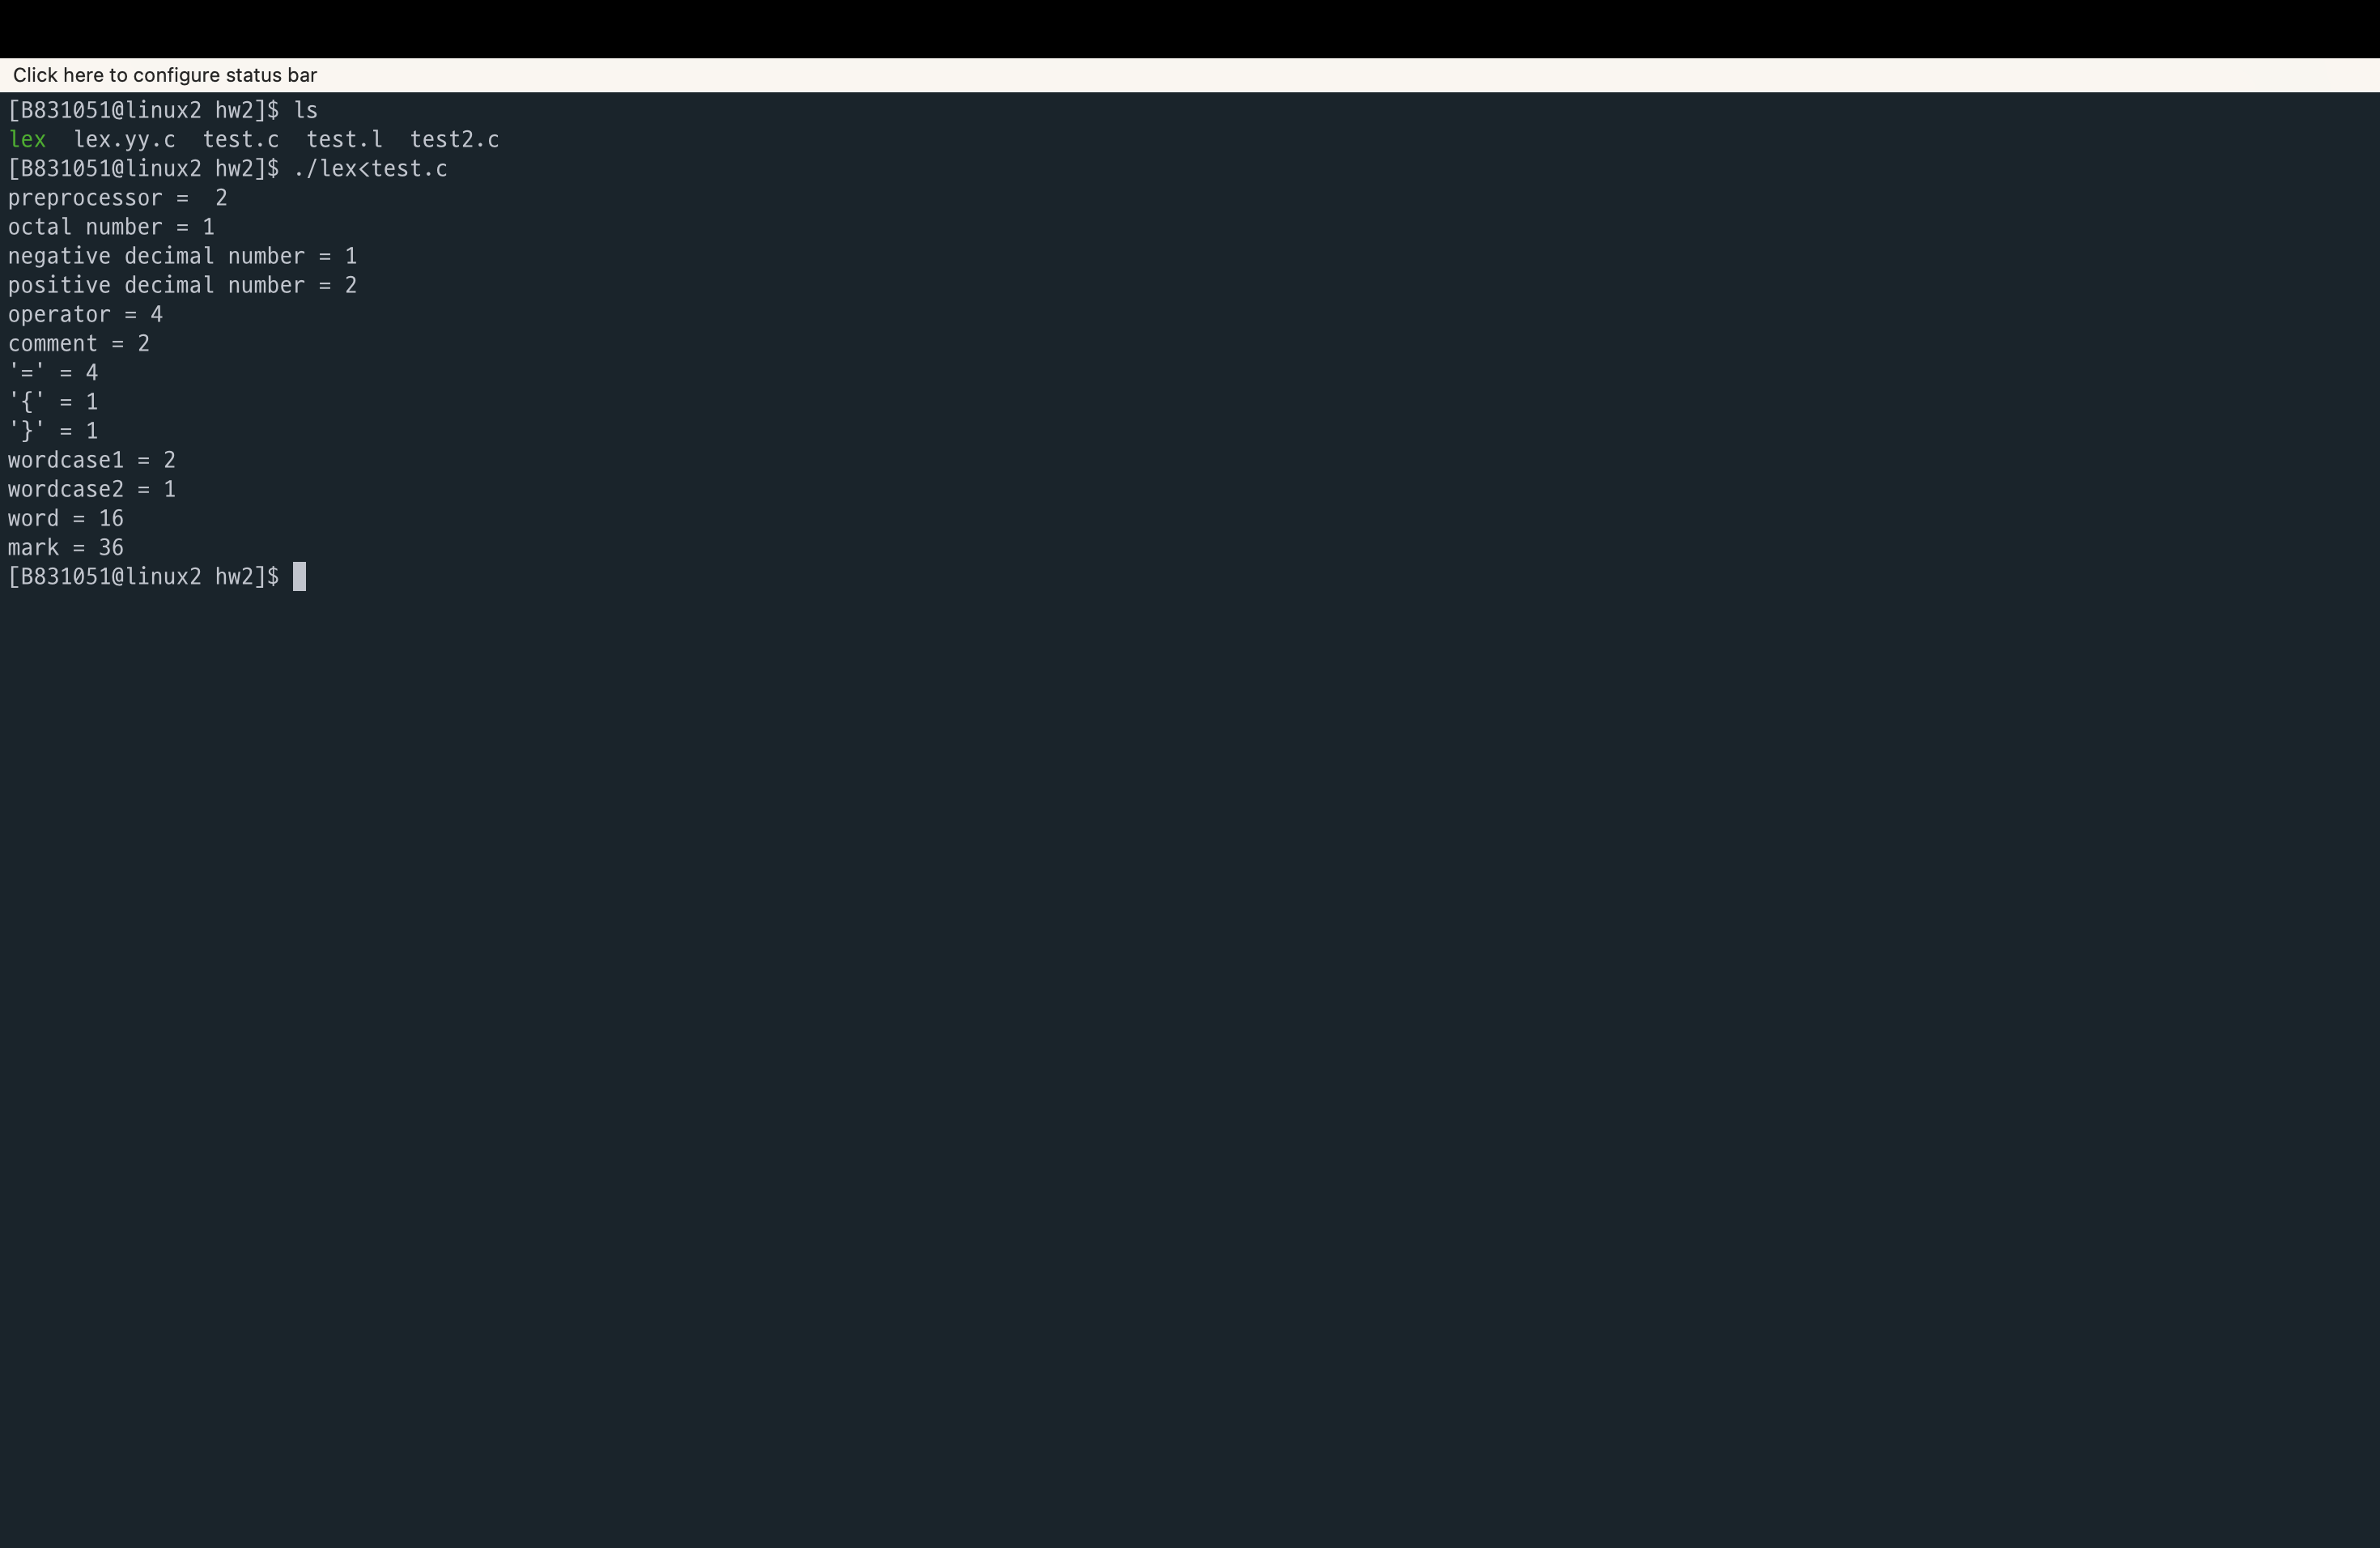
\includegraphics[width=0.7\textwidth]{hw2_result_screenshot.png}
    \caption{SeungWan}
    \label{fig:result_screenshot}
\end{figure}

\section{Code \& Comments}
\begin{verbatim}
    %{
/*정의절의 시작*/
#include <stdio.h>
int preprocessornum=0;//전처리기의 개수를 의미
int octalnum=0;//8진수의 개수를 의미
int negadecnum=0;//10진수 중 음수를 의미
int postdecnum=0;//10진수 중 양수를 의미
int operatornum=0;//연산자의 개수를 의미
int commentnum=0;//주석의 개수를 의미
int equalnum=0;//'='의 개수를 의미
int leftcurlybracenum=0;//'{'의 개수를 의미
int rightcurlybracenum=0;//'}'의 개수를 의미
int wordcase1=0;//p가 2번만 들어간 단어의 개수를 의미
int wordcase2=0;//e로 시작하고 마지막 글자가 m인 단어의 개수를 의미
int word=0;//그 이외의 단어 개수를 의미
int mark=0;//위에서 포함되지 않는 단어의 개수를 의미
%}
%%
	/*규칙절 정의 시작*/
#include|#define	{preprocessornum++;}
\{	{leftcurlybracenum++;}
\}	{rightcurlybracenum++;}
0[0-9]+	{octalnum++;}
-[0-9]+	{negadecnum++;}//음수
[0-9]+	{postdecnum++;}
\/{2}.*	{commentnum++;}
\/\*(\n)*.*(\n)*\*\/	{commentnum++;}
%[a-z]	{operatornum++;word++;}
\+|-|\*|%	{operatornum++;}//산술연산자
\|\||&&|!	{operatornum++;}//논리연산자
==|!=	{operatornum++;}//관계연산자
\+\+|--	{operatornum++;}
,	{operatornum++;}
\*|&	{operatornum++;}
\[[0-9]+\]	{mark+=3;}
[a-zA-Z]*p[a-zA-Z]*p[a-zA-Z]*p[a-zA-Z]*	{word++;}
[a-zA-Z]*p[a-zA-Z]*p[a-zA-Z]*	{wordcase1++;}
e[a-zA-Z]*m	{wordcase2++;}
=	{equalnum++;}
[a-zA-Z]+	{word++;} 
\n	;
.	{mark++;}
%%
int main()
{
	yylex();
	printf("preprocessor =  %d\n",preprocessornum);
	printf("octal number = %d\n",octalnum);
	printf("negative decimal number = %d\n",negadecnum);
	printf("positive decimal number = %d\n",postdecnum);
	printf("operator = %d\n",operatornum);
	printf("comment = %d\n",commentnum);
	printf("'=' = %d\n",equalnum);
	printf("'{' = %d\n",leftcurlybracenum);
	printf("'}' = %d\n",rightcurlybracenum);
	printf("wordcase1 = %d\n",wordcase1);
	printf("wordcase2 = %d\n",wordcase2);
	printf("word = %d\n",word);
	printf("mark = %d\n",mark);
	return 0;
}
int yywrap()
{
	return 1;
}

\end{verbatim}

Comment
\newline
1. 먼저 정의부에서는 주석에 포함된 바와 같이 출력을 위한 헤더인 stdio.h와 추후에 결과값 출력을 위한 변수들읠 정의 및 선언해주었습니다. 코드의 주석에 변수들의 의미가 나타나 있습니다.
\newline
2. 다음으로 본 코드의 핵심인 규칙절입니다. 헤더파일을 불러오고 전처리기를 통해서 변수를  처리하는 기능의 preprocessor는 #include와 #define을 통해 pattern을 명시했습니다. 이에 따라 전처리기 변수의 개수가 하나씩 증가됩니다. 그 다음에 위치한 중괄호 2개는 본 위치에 올 필요까지는 없지만 미리 선제적으로 정해주었습니다. 단, 두 중괄호 기호는 그 자체로는 정규표현식에서 의미가 있기에 슬래쉬를 사용하여 메타 character로써의 표기를 확실하게 해주었습니다.8진수는 0부터 시작한다는 특성을 가지고 이와 음수, 양의 정수는 1개 이상의 decimal한 수가 와야 하므로 1회 이상의 반복을 의미하는 + 정규표현을 통해 이를 나타냈습니다. 다음으로 굉장히 중요한 주석의 처리입니다. 과제의 명세서를 보면 주석의 내용은 count되지 않으므로 이를 잘 구현해야 합니다. 먼저, //주석의 경우에는 슬래쉬를 이용해 /자체를 나타낸다는 것을 명시해주고 {2}를 통해 정확히 2회만 쓰인다는 것을 나타냈습니다. 주석의 경우에 내용이 딱히 없을 수 있으므로 1줄짜리 주석인 //는 어떤 것이든 0회 이상 올 수 있다는 .*를 통해 나타냅니다. 다음으로 여러 줄의 주석을 표현할 수 있는 /**/ 역시 비슷하게 구현합니다. 다만, 개행문자가 올수도 있고 오지 않을 수도 있다는 뜻에서 이 역시 asterisk를 통해 표현했습니다. 이러한 방식을 통하면 주석의 내용은 count되지 않고 넘어갈 수 있습니다. 다음으로 매우 중요한 연산자의 처리입니다. 다만, 과제의 명세에 나온 바와 같이 \%d와 같은 문자는 각각 연산자와 단어로 처리되기에 연산자보다 위에 규칙을 정해줌으로써 우선순위를 높였습니다. 연산자들을 정의할 때 산술, 논리, 관계 증감, 콤마, 포인터 등을 구현할 때 메타 캐릭터들을 적절히 활용함으로 컴파일에 문제가 없게 합니다. 다음으로 본 과제의 하이라이트라고도 말할 수 있는 pp 단어의 처리입니다. 과제의 명세를 보면 정확히 p가 2번 들어간 단어만 wordcase1으로 처리해줘야 합니다. 저는 3개의 상의 p를 가진 단어를 '먼저' 처리해줌으로써 2번만 들어간 단어를 안전하게 처리했습니다. 정규표현식은 본 보고서에 첨부한 코드를 보면 알 수 있습니다. 또한 e로 시작하고 m으로 끝나는 단어는 e와 m을 앞과 뒤에 놓고 가운데에 어떠한 알파벳이든지 0회 이상 올 수 있다는 표현으로 나타냅니다(하지만 이는 특수 문자를 이용해 구현할 수도 있습니다). 마지막으로 남은 단어들을 의미하는 것들은 따로 처리하고 어디에도 해당되지 않는 공백, 세미콜론 등의 문자들은 mark로 처리합니다. 
\end{document}


